\clearpage
%//==============================--@--==============================//%
\subsection*{\underline{3.2} Considere o circuito RLC-série, com frequência de ressonância $\mathbf{f_0 = 60}\ \text{kHz}$ e admita que o valor estimado do coeficiente de auto-indução da bobina é $\mathbf{L = 3.0}\ \text{mH}$.}
%//==============================--A--==============================//%
\subsubsection*{(a) Determine o valor da capacidade C tal que o circuito esteja em ressonância à frequência $f_0$ indicada.}
\label{subsubsec_a}
\paragraph{Resposta:}
De acordo com as derivações e conclusões da alínea anterior, podemos imediatamente verificar que $\omega_0 L = \dfrac{1}{\omega_0 C}$. Pelo que, naturalmente, concluímos a expressão em ordem à incógnita:

$$
C = \frac{1}{\omega_0^2 L} \approx 2.345\ \text{nF}
$$

%//==============================--B--==============================//%
\subsubsection*{(b) Trace duas curvas da corrente normalizada, $I_n$, em função da frequência normalizada. Para cada um dos valores de $R=R_S$, determine as frequências das situações de meia potência $f_1$ e $f_2$, e determine, para cada caso, a largura de banda em valores absolutos $\Delta f$. Verifique (10).}
\label{subsubsec_b}
\paragraph{Resposta:}
Tendo em conta a frequência de ressonância $f_0 = 60\ \text{kHz}$ e o intervalo de frequências a que nos restringimos, i.e., $f \in \left[20; 90\right]\ \text{kHz}$, segue-se que a frequência normalizada ($f_n = \dfrac{f}{f_0}$) é delimitada no seguinte
intervalo: $f_n \in \left[\frac{1}{3}; \frac{3}{2}\right]$. 

\def\varQR{(2*pi*1.8)^2}
\def\varQRR{(2*pi*0.45)^2}
\def\fnum{-1/(2*2*pi*1.8)+sqrt(1/(4*(2*pi*1.8)^2)+1)}
\def\fndois{1/(2*2*pi*1.8)+sqrt(1/(4*(2*pi*1.8)^2)+1)}
\def\fntres{-1/(2*2*pi*0.45)+sqrt(1/(4*(2*pi*0.45)^2)+1)}
\def\fnquatro{1/(2*2*pi*0.45)+sqrt(1/(4*(2*pi*0.45)^2)+1)}
\begin{figure}[!h]  
    \begin{subfigure}[b]{0.45\textwidth}
    \centering
    \resizebox{1\textwidth}{!}{%
        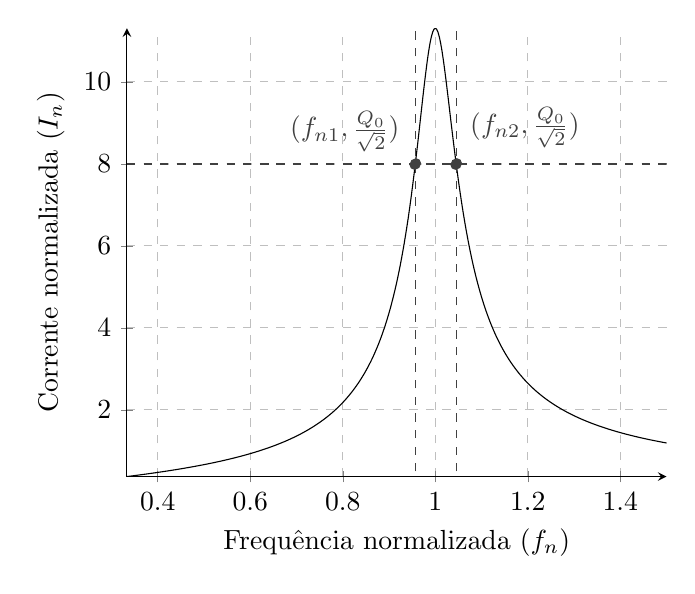
\begin{tikzpicture}
            \begin{axis}[
                axis lines = left,
                xlabel = {Frequência normalizada ($f_n$)},
                ylabel = {Corrente normalizada ($I_n$)},
                grid style=dashed,
                grid=major
            ]

            \addplot [
                domain=(1/3):(3/2), 
                samples=400, 
                color=black,
            ]
            { 1/sqrt( 1/(\varQR) + (x-1/x)^2 )};
            
            \addplot[
                domain=(1/3):(3/2), 
                samples=300, 
                color=darkgray,
                dashed
            ]
            {2*pi*1.8/sqrt(2)};
            
            \addplot [only marks,mark=*,dashed,color=darkgray] coordinates { (\fnum,2*pi*1.8/sqrt(2)};
            \node[label={160:{\color{darkgray} $(f_{n1},\frac{Q_0}{\sqrt{2}})$}},inner sep=2pt] at (0.956757,7.997189) {};
            
            \addplot [only marks,mark=*,dashed,color=darkgray] coordinates { (\fndois,2*pi*1.8/sqrt(2)};
            \node[label={55:{\color{darkgray} $(f_{n2},\frac{Q_0}{\sqrt{2}})$}},inner sep=2pt] at (1.045186,7.997189) {};
            
            \addplot +[mark=none,color=darkgray,dashed] coordinates {(\fnum, 0.5) (\fnum, 2*pi*1.8)};
            
            \addplot +[mark=none,color=darkgray,dashed] coordinates {(\fndois, 0.5) (\fndois, 2*pi*1.8)};
            
            %\addlegendentry{}
            \end{axis}
        \end{tikzpicture}
    }%
    \caption{Caso com $R=R_S=100\ \Omega$}
    \end{subfigure}
    \hfill
    \begin{subfigure}[b]{0.45\textwidth}
    \centering
    \resizebox{1\textwidth}{!}{%
        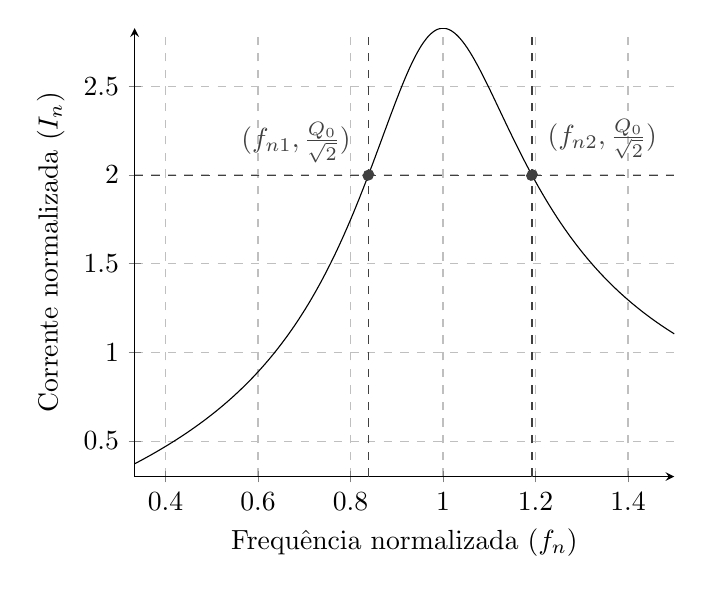
\begin{tikzpicture}
            \begin{axis}[
                axis lines = left,
                xlabel = {Frequência normalizada ($f_n$)},
                ylabel = {Corrente normalizada ($I_n$)},
                grid style=dashed,
                grid=major
            ]

            \addplot [
                domain=(1/3):(3/2), 
                samples=400, 
                color=black,
            ]
            { 1/sqrt( 1/(\varQRR) + (x-1/x)^2 )};
            
            \addplot[
                domain=(1/3):(3/2), 
                samples=300, 
                color=darkgray,
                dashed
            ]
            {2*pi*0.45/sqrt(2)};
            
            \addplot [only marks,mark=*,dashed,color=darkgray] coordinates { (\fntres,2*pi*0.45/sqrt(2)};
            \node[label={160:{\color{darkgray} $(f_{n1},\frac{Q_0}{\sqrt{2}})$}},circle,inner sep=2pt] at (0.838677,1.999297) {};

            \addplot [only marks,mark=*,dashed,color=darkgray] coordinates { (\fnquatro,2*pi*0.45/sqrt(2)};
            \node[label={45:{\color{darkgray} $(f_{n2},\frac{Q_0}{\sqrt{2}})$}},circle,inner sep=2pt] at (1.192354,1.999297) {};
            
            \addplot +[mark=none,color=darkgray,dashed] coordinates {(\fntres, 0.3) (\fntres, 2*pi*0.45)};
            
            \addplot +[mark=none,color=darkgray,dashed] coordinates {(\fnquatro, 0.3) (\fnquatro, 2*pi*0.45)};
            %\addlegendentry{}
            \end{axis}
        \end{tikzpicture}
    }%
    \caption{Caso com $R=R_S=400\ \Omega$}
    \end{subfigure}
\caption{Curvas de corrente normalizada para os dois valores possíveis da resistência (com os respectivos pontos de meia potência normalizados).} \label{fig:curvas_ressonancia} 
\end{figure}

$$
R=100\ \Omega:
\begin{cases}
    f_{n1} = 0.956757\\
    f_{n2} = 1.045186
\end{cases}
\implies \Delta f_n = 0.088419 \implies \Delta f = 5305\ \text{Hz}
$$

$$
R=400\ \Omega:
\begin{cases}
    f_{n1} = 0.838677\\
    f_{n2} = 1.192354
\end{cases}
\implies \Delta f_n = 0.353678 \implies \Delta f = 21220\ \text{Hz}
$$

Nas situações distintas observa-se:

$$
R=100\ \Omega:
\begin{cases}
    Q_0 = 11.309734\\
    \Delta f_n = 0.088419
\end{cases}
\land\
R=400\ \Omega:
\begin{cases}
    Q_0 = 2.827433\\
    \Delta f_n = 0.353678
\end{cases}
$$

Pelo que, naturalmente se verifica a relação enunciada $\Delta f_n = \dfrac{1}{Q_0}$.

$$
R=100\ \Omega:
\begin{cases}
    \dfrac{1}{Q_0} = 0.088419\\
    \Delta f_n = 0.088419
\end{cases}
\land\
R=400\ \Omega:
\begin{cases}
    \dfrac{1}{Q_0} = 0.353678\\
    \Delta f_n = 0.353678
\end{cases}
$$

$$\therefore \Delta f_n = \frac{1}{Q_0}$$
\hfill \ensuremath{\Box}
%//==============================--C--==============================//%
\subsubsection*{(c) Para o caso $R_S = 100\ \Omega$, $U_{gef} = 1\ \text{V}$ e tomando $C$ o valor determinado em \hyperref[subsubsec_a]{(a)}, calcule os valores eficazes e desfasagens da corrente $i$ e das tensões no condensador, $u_C$, na bobina, $u_L$, e na resistência, $u_R$, para a frequência de ressonância, $f_0$, bem como para as frequências $f_1$ e $f_2$.}
\label{subsubsec_c}
\paragraph{Resposta:}
Por aplicação direta da Lei de Indução, obtemos as seguintes relações cruciais à análise:

\begin{equation}
    \label{eq1}
    \begin{cases}
        u_G = u_R + u_L + u_C = iR + L\dfrac{di}{dt} + \dfrac{1}{C}\int i\,dt\\
        \bar{U}_G = \bar{U}_R + \bar{U}_L + \bar{U}_C = \bar{I}R + j\omega L\bar{I} + \dfrac{1}{j\omega C}\bar{I}
    \end{cases}
\end{equation}

Salientando novamente, da \hyperref[subsection3_1]{alínea \underline{3.1}}, a impedância equivalente observada em ressonância é puramente resistiva para o circuito RLC-série, pelo que este é o caso mais trivial:

$$
f_0 :
\begin{cases}
\bar{Z}_{eq} = R + j(\omega_0 L - \frac{1}{\omega_0 C}) = 100\ \Omega \implies \bar{I} = \dfrac{\bar{U}_G}{\bar{Z}_{eq}} = \dfrac{U_{Gef}\sqrt{2}\ e^{j0}}{R} = \dfrac{\sqrt{2}}{100} e^{j0}\ \text{A}\\
\bar{U}_R = \bar{I}R = \sqrt{2}\ e^{j0}\ \text{V}\\
\bar{U}_L = j\omega_0 L \bar{I} = 11.310\sqrt{2}\ e^{j\frac{\pi}{2}}\ \text{V}\\
\bar{U}_C = \dfrac{1}{j\omega_0 C}\bar{I} = 11.310\sqrt{2}\ e^{-j\frac{\pi}{2}}\ \text{V}
\end{cases}
$$

Para as seguintes frequências, $f_1$ e $f_2$, o procedimento será o mesmo, no entanto, note-se que a impedância equivalente já \textbf{não será} puramente resistiva, o que se traduz numa corrente $i$ com fase diferente da de $u_G$. Da alínea \hyperref[subsubsec_b]{\underline{3.2} (b)} temos:

$$
\begin{cases}
    f_{n1} = 0.956757\\
    f_{n2} = 1.045186
\end{cases}
\implies
\begin{cases}
    f_1 = 57.405\ \text{kHz}\\
    f_2 = 62.711\ \text{kHz}
\end{cases}
\implies
\begin{cases}
    \omega_1 = 360.891\ \text{krad\ $s^{-1}$}\\
    \omega_2 = 394.025\ \text{krad\ $s^{-1}$}
\end{cases}
$$

\clearpage
Deste modo, juntamente com as ferramentas de \hyperref[eq1]{(1)}, rapidamente chegamos a:

$$
f_1 :
\begin{cases}
    \bar{Z}_{eq} = 140.685\ e^{-j 0.780}\ \Omega\\
    \bar{I} = \dfrac{\bar{U}_G}{\bar{Z}_{eq}} =  \dfrac{\sqrt{2}}{140.685}e^{j0.780}\ \text{A}\\
    \bar{U}_R = \bar{I}R = 0.710\sqrt{2}\ e^{j0.780}\ \text{V}\\
    \bar{U}_L = j\omega_1 L \bar{I} = 7.696\sqrt{2}\ e^{j2.351}\ \text{V}\\
    \bar{U}_C = \dfrac{1}{j\omega_1 C}\bar{I} = 8.399\sqrt{2}\ e^{-j0.791}\ \text{V}
\end{cases}
f_2 :
\begin{cases}
    \bar{Z}_{eq} = 141.287\ e^{j0.784}\ \Omega\\    
    \bar{I} = \dfrac{\bar{U}_G}{\bar{Z}_{eq}} = \dfrac{\sqrt{2}}{141.287}e^{-j0.784}\ \text{A}\\
    \bar{U}_R = \bar{I}R = 0.708\sqrt{2}\ e^{-j0.784}\ \text{V}\\
    \bar{U}_L = j\omega_2 L \bar{I} = 8.366\sqrt{2}\ e^{j0.787}\ \text{V}\\
    \bar{U}_C = \dfrac{1}{j\omega_2 C}\bar{I} = 7.660\sqrt{2}\ e^{-j2.355}\ \text{V}
\end{cases}
$$

Sintéticamente, em tabela:

\begin{table}[ht]
    \centering
    \caption{Valores eficazes e desfasagens das grandezas consideras.}
    \label{tab1}
    \begin{tabular}{SSSSSSSSS}
        \toprule
        $f$ & $I_{ef}/\text{mA}$ & $\alpha_I/^{\circ}$ & $U_{Ref}/\text{V}$ & $\alpha_R/^{\circ}$ & $U_{Lef}/\text{V}$ & $\alpha_L/^{\circ}$ & $U_{Cef}/\text{V}$ & $\alpha_C/^{\circ}$ \\ \midrule
        $f_0$  & 10 & 0 & 1 & 0 & 11.310 & 90 & 11.310 & -90\\
        $f_1$  & 7.108 & 44.690 & 0.710 & 44.690 & 7.696 & 134.702 & 8.399 & -45.320\\
        $f_2$ & 7.078 & -44.920 & 0.708 & -44.920 & 8.366 & 45.092 & 7.660 & -135.932\\ \bottomrule
    \end{tabular}
\end{table}
%//==============================--D--==============================//%
\subsubsection*{(d) Para as condições da alínea anterior e para cada uma dessas três frequências trace os correspondentes diagramas vectoriais de tensão.}
\paragraph{Resposta:}
Apresentam-se, em seguida, os diagramas vectoriais como enunciado:

%\iffalse
\begin{figure}[H]
    \centering
    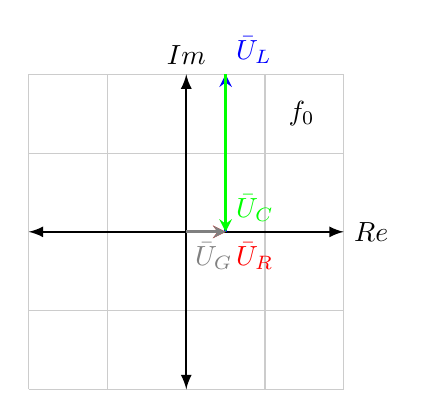
\begin{tikzpicture}[>=latex]
    \node[text width=1cm] at (1.8,1.5) {$f_0$};
        %{
            \draw[thin,gray!40] (-2,-2) grid (2,2);
            \draw[<->,thick,black] (-2,0) -- (2,0) node [right] {$\mathbb{R}e$};
            \draw[<->,thick,black] (0,-2) -- (0,2) node [above] {$\mathbb{I}m$};
        %} plano imaginário
        \draw[line width=1pt,blue,-stealth](0.5,0)--(0.5,2) node[anchor=south west]{$\boldsymbol{\bar{U}_L}$};
        \draw[line width=1pt,green,-stealth](0.5,2)--(0.5,0) node[anchor=south west]{$\boldsymbol{\bar{U}_C}$}; 
        \draw[line width=1pt,red,-stealth](0,0)--(0.5,0) node[anchor=north west]{$\boldsymbol{\bar{U}_R}$}; 
        \draw[line width=1pt,gray,-stealth](0,0)--(0.5,0) node[anchor=north, xshift=-0.15cm]{$\boldsymbol{\bar{U}_G}$};
    \end{tikzpicture}\\
    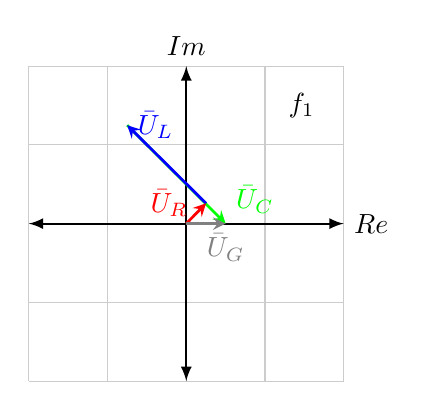
\begin{tikzpicture}[>=latex]
    \node[text width=1cm] at (1.8,1.5) {$f_1$};
        %{
            \draw[thin,gray!40] (-2,-2) grid (2,2);
            \draw[<->,thick,black] (-2,0) -- (2,0) node [right] {$\mathbb{R}e$};
            \draw[<->,thick,black] (0,-2) -- (0,2) node [above] {$\mathbb{I}m$};
        %} plano imaginário
        \draw[line width=1pt,green,-stealth](-0.75,1.25)--(0.5,0) node[anchor=south west]{$\boldsymbol{\bar{U}_C}$};
        \draw[line width=1pt,blue,-stealth](45.7:0.36)--(-0.75,1.25) node[anchor=west]{$\boldsymbol{\bar{U}_L}$}; 
        \draw[line width=1pt,red,-stealth](0,0)--(45.7:0.36) node[left,xshift=-0.1cm]{$\boldsymbol{\bar{U}_R}$}; 
        \draw[line width=1pt,gray,-stealth](0,0)--(0.5,0) node[anchor=north]{$\boldsymbol{\bar{U}_G}$};
    \end{tikzpicture}
    \qquad
    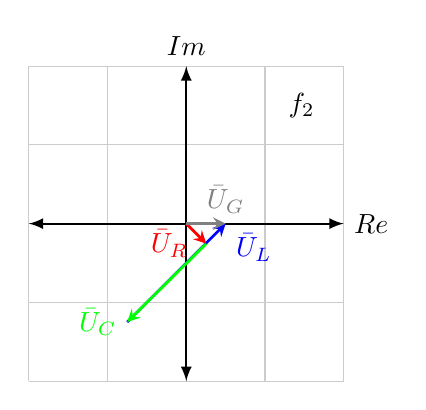
\begin{tikzpicture}[>=latex]
    \node[text width=1cm] at (1.8,1.5) {$f_2$};
        %{
            \draw[thin,gray!40] (-2,-2) grid (2,2);
            \draw[<->,thick,black] (-2,0) -- (2,0) node [right] {$\mathbb{R}e$};
            \draw[<->,thick,black] (0,-2) -- (0,2) node [above] {$\mathbb{I}m$};
        %} plano imaginário
        \draw[line width=1pt,blue,-stealth](-0.75,-1.25)--(0.5,0) node[anchor=north west]{$\boldsymbol{\bar{U}_L}$}; 
        \draw[line width=1pt,green,-stealth](-44.9:0.36)--(-0.75,-1.25) node[anchor=east]{$\boldsymbol{\bar{U}_C}$};
        \draw[line width=1pt,red,-stealth](0,0)--(-44.9:0.36) node[left,xshift=-0.1cm]{$\boldsymbol{\bar{U}_R}$}; 
        \draw[line width=1pt,gray,-stealth](0,0)--(0.5,0) node[anchor=south]{$\boldsymbol{\bar{U}_G}$};
    \end{tikzpicture}
    \caption{Diagramas vectoriais de tensão para $f_0$, $f_1$ e $f_2$.}
\end{figure}
%\fi
%//==============================--@--==============================//%
